% Chapter 5: System Implementation
\chapter{System Implementation}

\section{Arduino Implementation}
The Arduino WiFi R4 serves as the central hardware controller, executing the washing cycle based on parameters retrieved from Firebase. The firmware is written in C++ using the Arduino IDE.

\subsection{Washing Machine Control Algorithm}
The firmware follows a structured sequence to manage the washing process autonomously. Upon receiving parameters from Firebase, the system initiates an initial drum rotation to balance the load, followed by automated detergent dispensing and water filling. The soak phase and main wash cycle are then executed, with support for additional rinse and spin cycles as specified by the user. The following flowchart details this operational logic.

\begin{figure}[H]
    \centering
    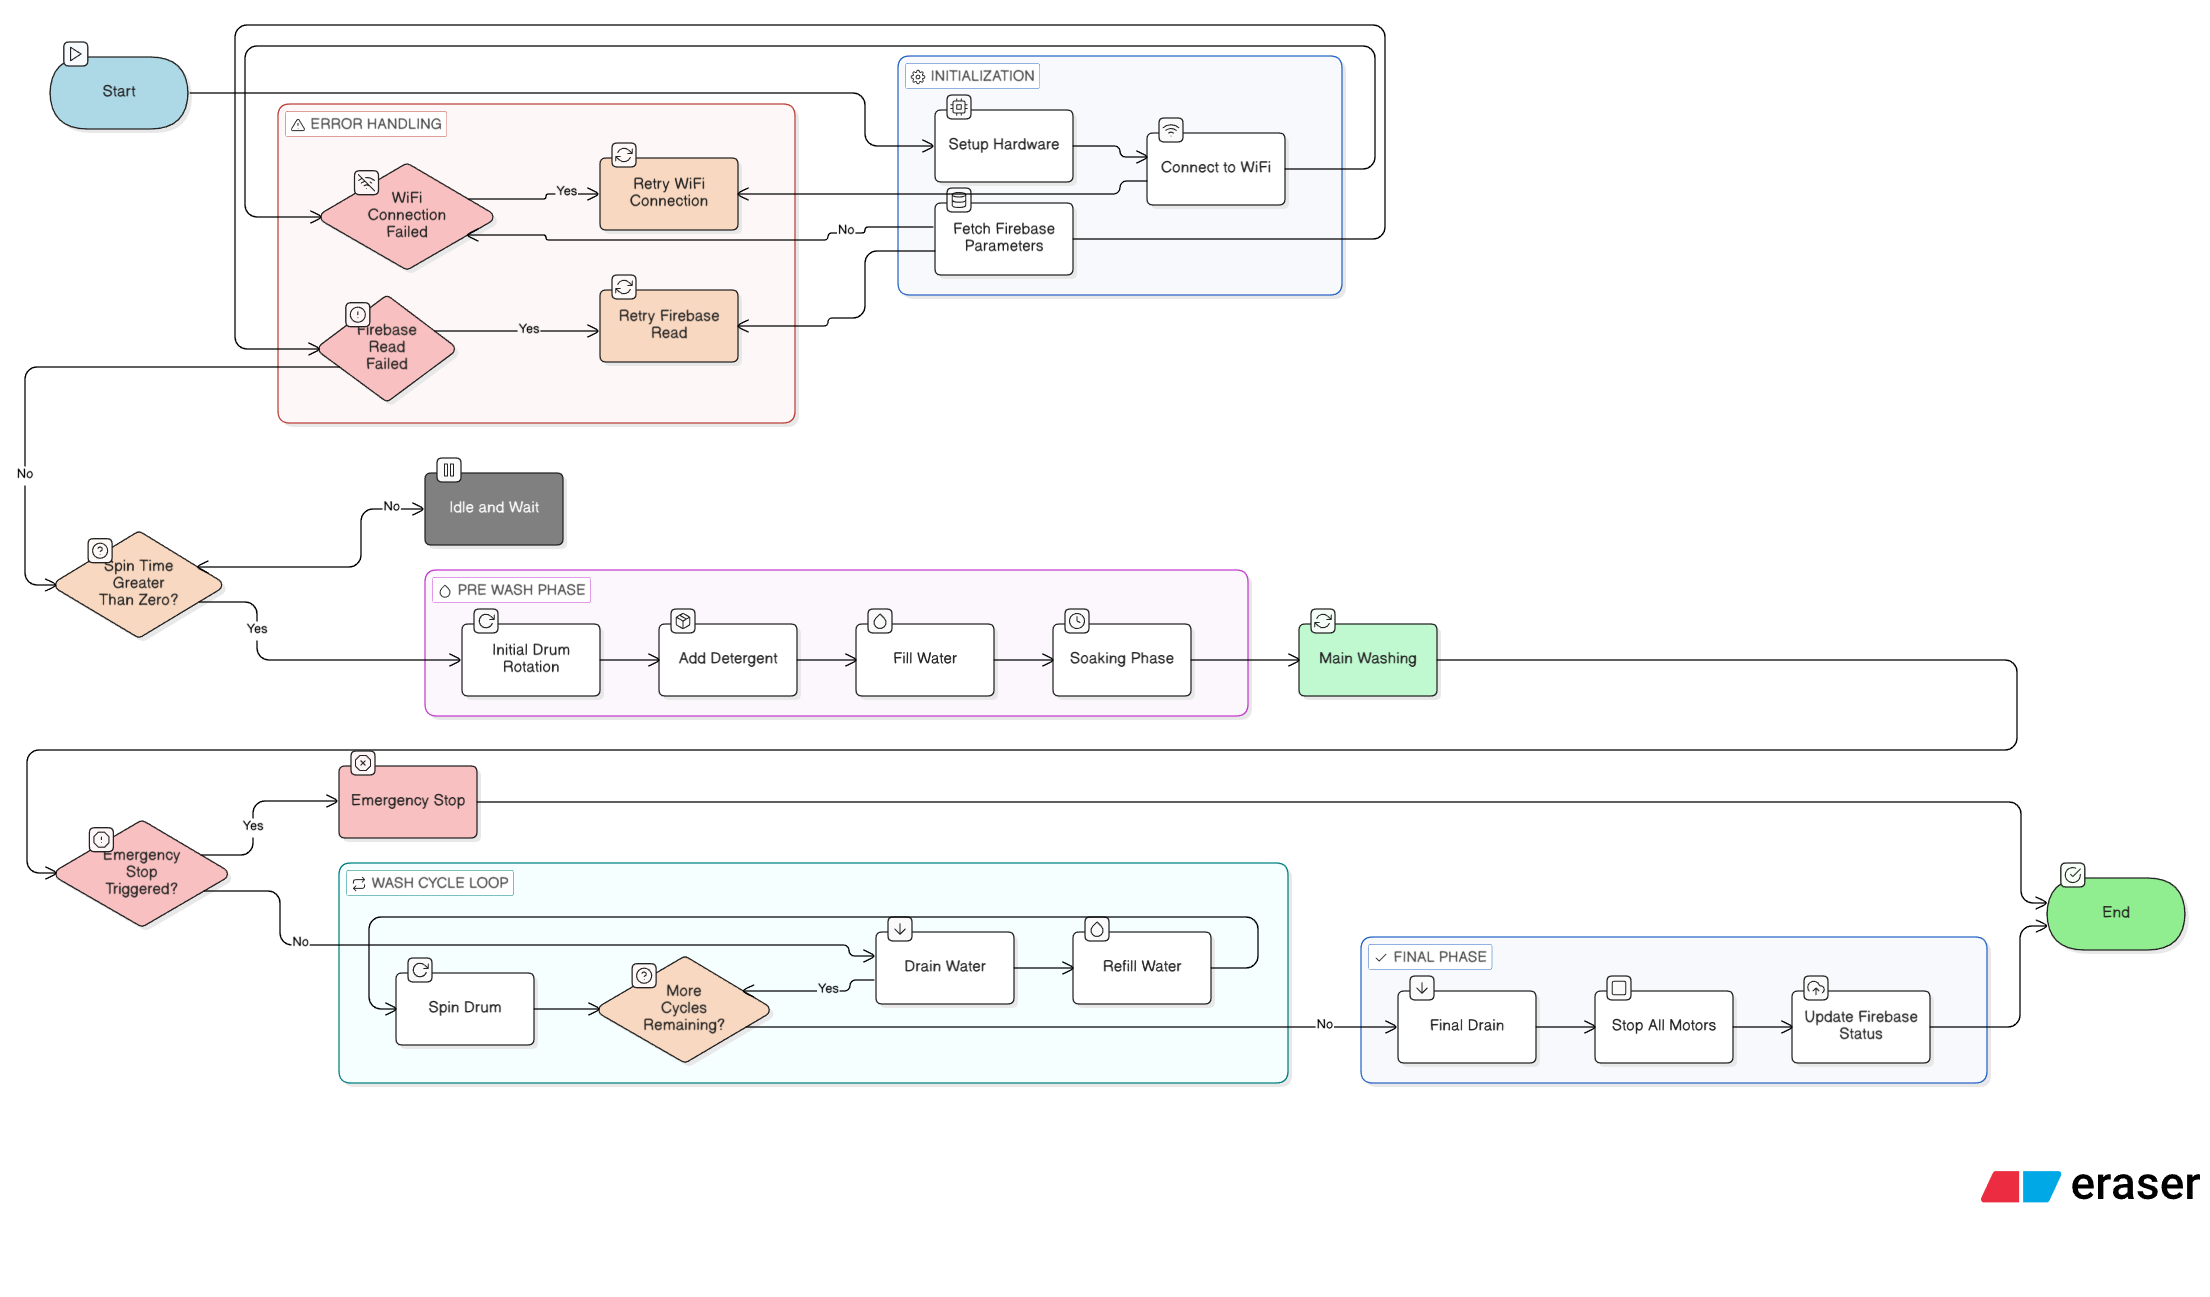
\includegraphics[width=1.0\textwidth]{img/c5WM_algorithm}
    \caption{Washing Machine Logic Flowchart}
    \label{fig:wm_algorithm}
\end{figure}

\subsection{Complete Arduino Code}

\begin{figure}[H]
    \centering
    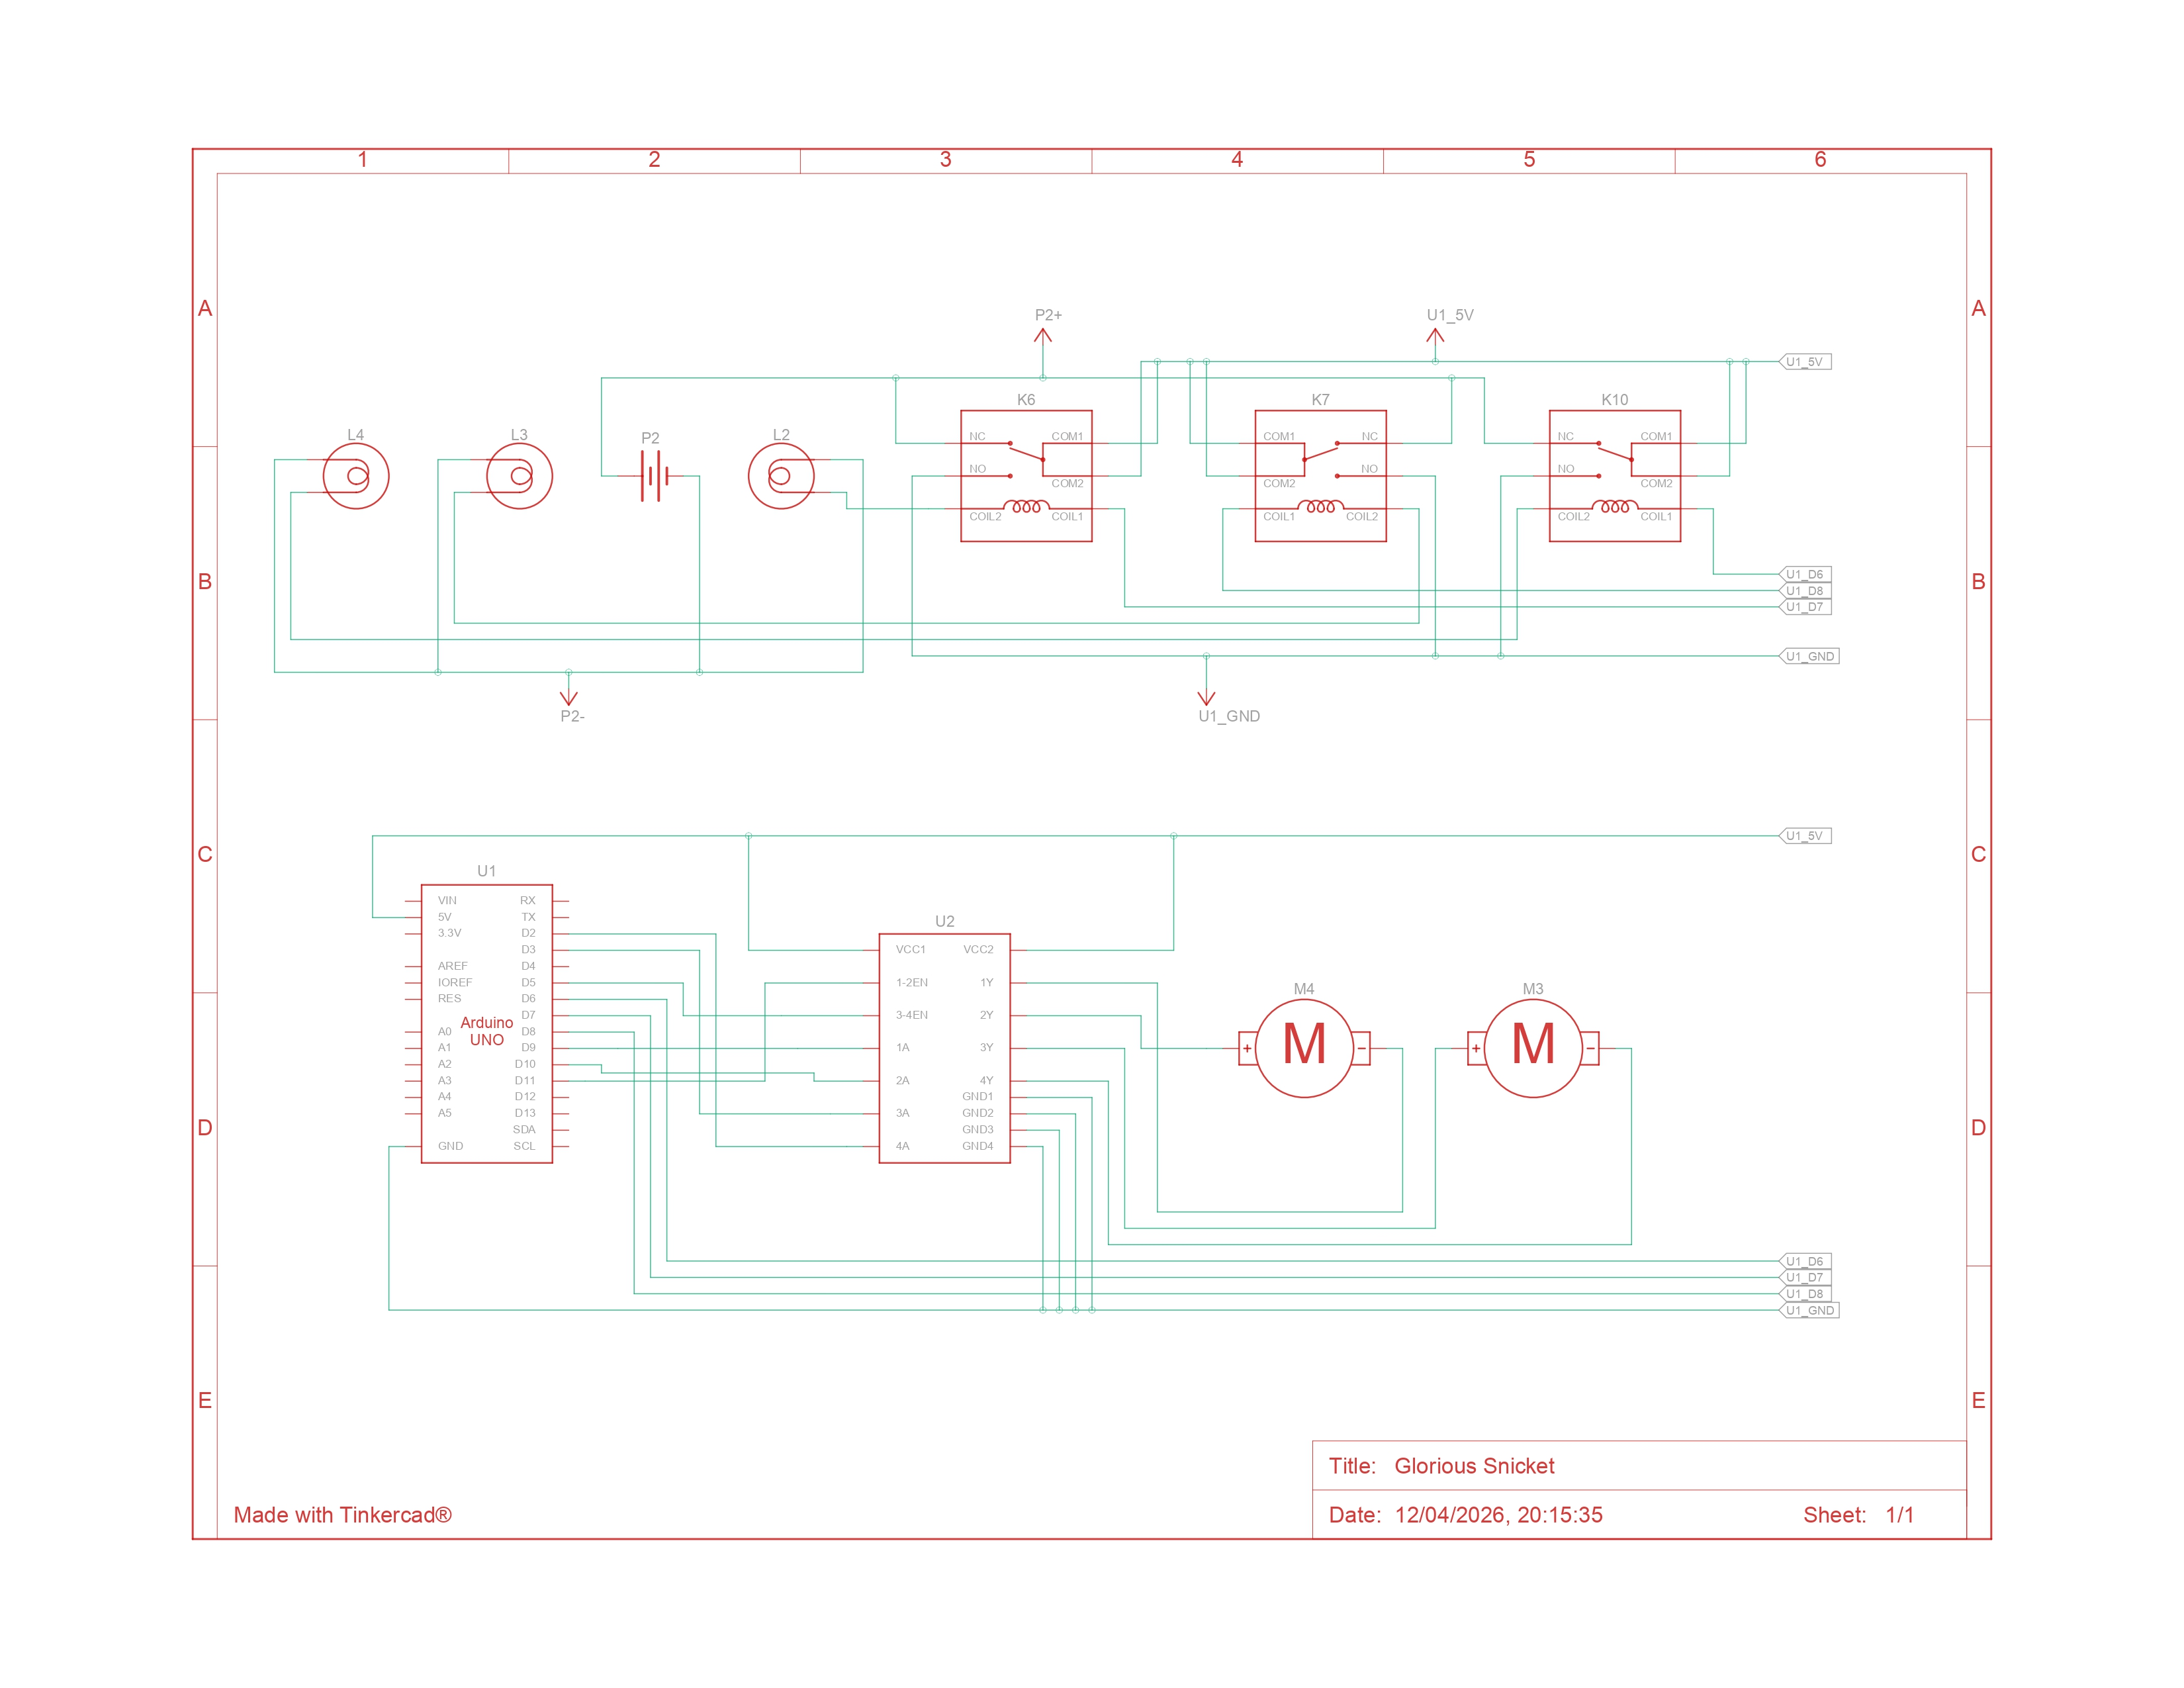
\includegraphics[width=0.9\textwidth]{img/c5diagram1}
    \caption{Circuit Diagram}
    \label{fig:arduino_ide}
\end{figure}

\begin{lstlisting}[language=C++, caption=Complete Arduino Firmware, label=lst:arduino_full]
#include "secrets.h"
#include <Firebase.h>
#include <WiFiS3.h>

// ================= Firebase =================
Firebase fb(REFERENCE_URL);

int detergent_amount = 0;   // ml
int soack_time = 0;         // sec
int spin_time = 0;          // sec
int wash_cycle = 0;         // count
int water_level = 0;        // liters

// ================= Drum =================
int CW = 7;
int CCW = 8;

// ================= Pump =================
int enPin = 5;
int pumpIn1 = 3;
int pumpIn2 = 2;

// Calibration
float a = 0.02218;
float b = -3.570;
int motorSpeed = 128;

// ================= Valves =================
int INLET = 6;

int outletIn1 = 9;
int outletIn2 = 10;
int outletEnA = 11;

// ================= Timing =================
unsigned long rotateRunTime = 5000;
unsigned long rotateStopTime = 2000;
unsigned long drainTime = 60000; // 1 min

// =====================================================
// SETUP
// =====================================================
void setup() {
  Serial.begin(115200);

  pinMode(CW, OUTPUT);
  pinMode(CCW, OUTPUT);

  pinMode(enPin, OUTPUT);
  pinMode(pumpIn1, OUTPUT);
  pinMode(pumpIn2, OUTPUT);

  pinMode(INLET, OUTPUT);

  pinMode(outletIn1, OUTPUT);
  pinMode(outletIn2, OUTPUT);
  pinMode(outletEnA, OUTPUT);

  stopDrum();
  stopPump();
  closeInletValve();
  stopOutletMotor();

  // -------- WiFi --------
  WiFi.begin(WIFI_SSID, WIFI_PASSWORD);
  while (WiFi.status() != WL_CONNECTED) {
    delay(500);
    Serial.print(".");
  }
  Serial.println("\nWiFi Connected");

  // -------- Firebase Read --------
  fb.getInt("detergent_amount", detergent_amount);
  fb.getInt("soack_time", soack_time);
  fb.getInt("spin_time", spin_time);
  fb.getInt("wash_cycle", wash_cycle);
  fb.getInt("water_level", water_level);

  Serial.println("Firebase Data Loaded");
}

// =====================================================
// LOOP
// =====================================================
void loop() {

  if (spin_time > 0) {

    Serial.println("===== WASH STARTED =====");

    float waterML = water_level * 1000.0;

    // STEP 1: Initial rotation
    rotateDrumForDuration(15000);

    // STEP 2: Add detergent
    dispense(detergent_amount);

    // STEP 3: Fill water
    fillWater(waterML);

    // STEP 4: Soak
    delay(soack_time * 1000UL);

    // STEP 5: MAIN WASH
    rotateDrumForDuration(spin_time * 1000UL);

    // ===============================
    //  EXTRA WASH CYCLES
    // ===============================
    for (int i = 0; i < wash_cycle; i++) {

      Serial.print("Cycle ");
      Serial.println(i + 1);

      // Drain
      openOutletValve();
      delay(drainTime);
      closeOutletValve();

      // Refill
      fillWater(waterML);

      // Spin again
      rotateDrumForDuration(spin_time * 1000UL);
    }

    // FINAL DRAIN
    openOutletValve();
    delay(drainTime);
    closeOutletValve();

    Serial.println("===== WASH COMPLETE =====");

    spin_time = 0; // prevent repeat
  }
}
\end{lstlisting}


\subsection{Motor Rotation Logic}
The motor control function implements the timed rotation pattern required for effective washing.

\begin{lstlisting}[language=C++, caption=Motor Rotation Control, label=lst:motor]
void rotateCW() {
  digitalWrite(CW, LOW);
  digitalWrite(CCW, HIGH);
}

void rotateCCW() {
  digitalWrite(CW, HIGH);
  digitalWrite(CCW, LOW);
}

void stopDrum() {
  digitalWrite(CW, HIGH);
  digitalWrite(CCW, HIGH);
}

void rotateDrumForDuration(unsigned long totalTime) {

  unsigned long startTime = millis();

  while (millis() - startTime < totalTime) {

    rotateCW();
    delay(rotateRunTime);

    stopDrum();
    delay(rotateStopTime);

    if (millis() - startTime >= totalTime) break;

    rotateCCW();
    delay(rotateRunTime);

    stopDrum();
    delay(rotateStopTime);
  }

  stopDrum();
}
\end{lstlisting}

\subsection{Detergent Dispenser Control}
The detergent pump is controlled using the linear regression equation derived from calibration.

\begin{lstlisting}[language=C++, caption=Detergent Dispensing Functions, label=lst:detergent]
void stopPump() {
  analogWrite(enPin, 0);
  digitalWrite(pumpIn1, LOW);
  digitalWrite(pumpIn2, LOW);
}

void dispense(float ml) {

  float cal_ml = ml * 0.41;
  float time_ms = (cal_ml - b) / a;

  if (time_ms < 0) time_ms = 0;

  analogWrite(enPin, motorSpeed);
  digitalWrite(pumpIn1, HIGH);
  digitalWrite(pumpIn2, LOW);

  delay((unsigned long)time_ms);

  stopPump();
}
\end{lstlisting}

\subsection{Water Inlet Control}

\begin{lstlisting}[language=C++, caption=Water Inlet Function, label=lst:water]
void openInletValve() {
  digitalWrite(INLET, LOW);
}

void closeInletValve() {
  digitalWrite(INLET, HIGH);
}

void fillWater(float ml) {

  unsigned long fillTime = (ml / 650.0) * 10000.0;

  openInletValve();
  delay(fillTime);
  closeInletValve();
}
\end{lstlisting}

\section{Linear Regression for Detergent Dispensing}
Precise detergent dispensing required empirical calibration to establish the relationship between pump activation time and dispensed volume.

\subsection{Calibration Data Collection}
Detergent volume was measured at 50ms intervals from 50ms to 2400ms. The data was recorded and is presented in Table~\ref{tab:calibration}.


\begin{table}[H]
    \centering
    \small
    \caption{Calibration Data}\label{tab:calibration}
    \begin{tabular}{|c|c|}
        \hline
        \textbf{Time (ms)} & \textbf{Volume (ml)} \\
        \hline
        50   & 0.0   \\
        100  & 0.0   \\
        150  & 0.0   \\
        200  & 0.5   \\
        250  & 2.0   \\
        300  & 3.0   \\
        350  & 4.5   \\
        400  & 5.0   \\
        450  & 6.0   \\
        500  & 7.5   \\
        550  & 8.5   \\
        600  & 9.75  \\
        650  & 10.25 \\
        700  & 11.5  \\
        750  & 12.0  \\
        800  & 13.0  \\
        850  & 15.0  \\
        900  & 16.5  \\
        950  & 18.0  \\
        1000 & 19.0  \\
        1050 & 20.0  \\
        1100 & 21.0  \\
        1200 & 23.0  \\
        1300 & 25.5  \\
        1400 & 26.5  \\
        1500 & 28.0  \\
        1600 & 30.0  \\
        1700 & 33.0  \\
        1800 & 35.5  \\
        1900 & 39.5  \\
        2000 & 41.5  \\
        2100 & 44.5  \\
        2200 & 46.0  \\
        2300 & 48.0  \\
        2400 & 50.5  \\
        \hline
    \end{tabular}
\end{table}
\newpage
\subsection{Linear Regression Analysis}
Using the method of least squares, the linear regression coefficients were calculated as follows:

\begin{align*}
\text{Number of observations } n &= 35 \\
\text{Sum of time } \Sigma x &= 42000 \\
\text{Sum of volume } \Sigma y &= 637.5 \\
\text{Sum of squares of time } \Sigma x^2 &= 63,\!700,\!000 \\
\text{Sum of products } \Sigma xy &= 1,\!047,\!750
\end{align*}

The slope \(a\) and intercept \(b\) are computed using the formulas:

\[
a = \frac{n \cdot \Sigma xy - \Sigma x \cdot \Sigma y}{n \cdot \Sigma x^2 - (\Sigma x)^2}
\]
\[
b = \frac{\Sigma y - a \cdot \Sigma x}{n}
\]

Substituting the values:

\vspace{-10pt}
\[
a = \frac{35 \times 1,\!047,\!750 - 42000 \times 637.5}{35 \times 63,\!700,\!000 - 42000^2} = 0.022175840697103585
\]
\vspace{-10pt}
\[
b = \frac{637.5 - a \times 42000}{35} = -3.5696873465881223
\]
\vspace{-10pt}
\begin{figure}[H]
    \centering
    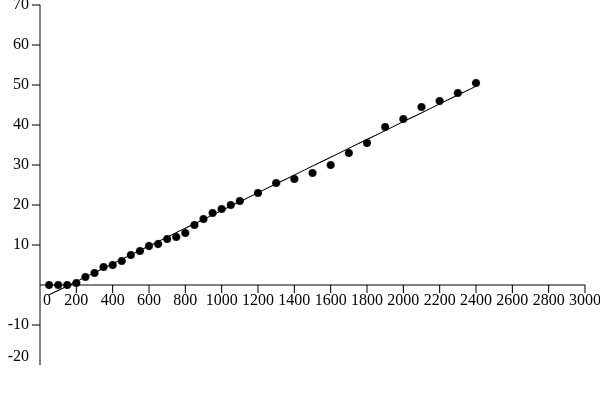
\includegraphics[width=0.7\textwidth]{img/c5diagram3}
    \caption{Volume vs Time Linear Regression Graph}
    \label{fig:regression_graph}
\end{figure}

\textbf{Regression Equation:}
\vspace{-12pt}
\[
\text{Volume (ml)} = 0.022176 \times \text{Time (ms)} - 3.569687
\]
\vspace{-12pt}
\begin{table}[H]
    \centering
    \small
    \setlength{\tabcolsep}{4pt}
    \begin{tabular}{|l|c|}
        \hline
        \textbf{Coefficient} & \textbf{Value} \\
        \hline
        \(a\) (slope)   & 0.022176 \\
        \(b\) (intercept)& -3.569687 \\
        \(R^2\) value    & 0.997 (approx.) \\
        \hline
    \end{tabular}
    \caption{Linear Regression Coefficients}
    \label{tab:coeff}
\end{table}

The high \(R^2\) value indicates excellent linear correlation, validating the linear model for precise dispensing control.

\subsection{Implementation in Arduino}
The derived equation is implemented in the Arduino code for real-time calculation. To find the time required for a desired volume, the equation is rearranged:
\vspace{-8pt}
\[
\text{Time (ms)} = \frac{\text{Volume} + 3.569687}{0.022176}
\]
\vspace{-8pt}
The Arduino function uses this formula with safety constraints as shown in section~\ref{lst:detergent}.
\section{API Implementation}
Two FastAPI services were implemented to handle fabric analysis and washing parameter calculation.
\subsection{FastAPI 1: Clothing Material Identifier}
\begin{figure}[H]
    \centering
    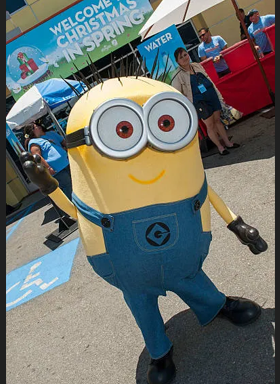
\includegraphics[width=0.7\textwidth]{img/c5diagram4}
    \caption{FastAPI 1 Implementation}
    \label{fig:fastapi1_code}
\end{figure}

\begin{lstlisting}[language=Python, caption=FastAPI 1 Code, label=lst:fastapi1]
from fastapi import FastAPI, File, UploadFile, HTTPException
from fastapi.responses import JSONResponse
import google.generativeai as genai
from PIL import Image
import io
import os
from typing import List
from pydantic import BaseModel

app = FastAPI(title="Clothing Material Identifier API")

# Configure Gemini API
genai.configure(api_key=os.getenv("GEMINI_API_KEY"))
model = genai.GenerativeModel('gemini-1.5-flash')

class FabricResponse(BaseModel):
    filename: str
    material_type: str
    fiber_category: str
    description: str
    dirt_level: int
    confidence_score: float

class BatchResponse(BaseModel):
    total_images: int
    results: List[FabricResponse]

@app.post("/predict/", response_model=BatchResponse)
async def predict_materials(files: List[UploadFile] = File(...)):
    results = []
    
    for file in files:
        # Read image
        image_data = await file.read()
        image = Image.open(io.BytesIO(image_data))
        
        # Construct prompt
        prompt = """Objective: Look at this photo of clothing.
1. Tell me the specific fabric name (like Cotton, Silk, Denim, Polyester).
2. Tell me if it's Natural, Synthetic, or Semi-synthetic.
3. Tell me how dirty it is on a scale of 1 to 5 using these criteria:
   Level 1: Clean/Light Use - No visible stains
   Level 2: Surface Soiled - Localized minor spots
   Level 3: Moderately Dirty - Visible sweat marks or multiple small stains
   Level 4: Heavily Soiled - Large deep-set stains covering >25% of surface
   Level 5: Emergency - Complete saturation with thick grime
4. Provide a 3-line description of the fabric properties.
Return the answer in strict JSON format with keys: material_type, fiber_category, description, dirt_level, confidence_score"""
        
        # Get response from Gemini
        response = model.generate_content([prompt, image])
        
        # Parse JSON response (simplified - actual implementation uses json.loads)
        import json
        result = json.loads(response.text)
        
        results.append({
            "filename": file.filename,
            "material_type": result["material_type"],
            "fiber_category": result["fiber_category"],
            "description": result["description"],
            "dirt_level": result["dirt_level"],
            "confidence_score": result["confidence_score"]
        })
    
    return {"total_images": len(results), "results": results}

@app.post("/feedback/")
async def submit_feedback(filename: str, correct_material: str):
    # Store feedback for model improvement
    # Implementation details here
    return {"message": "Feedback received"}
\end{lstlisting}

\newpage
\subsection{API Documentation}
FastAPI automatically generates interactive API documentation.

\begin{figure}[H]
    \centering
    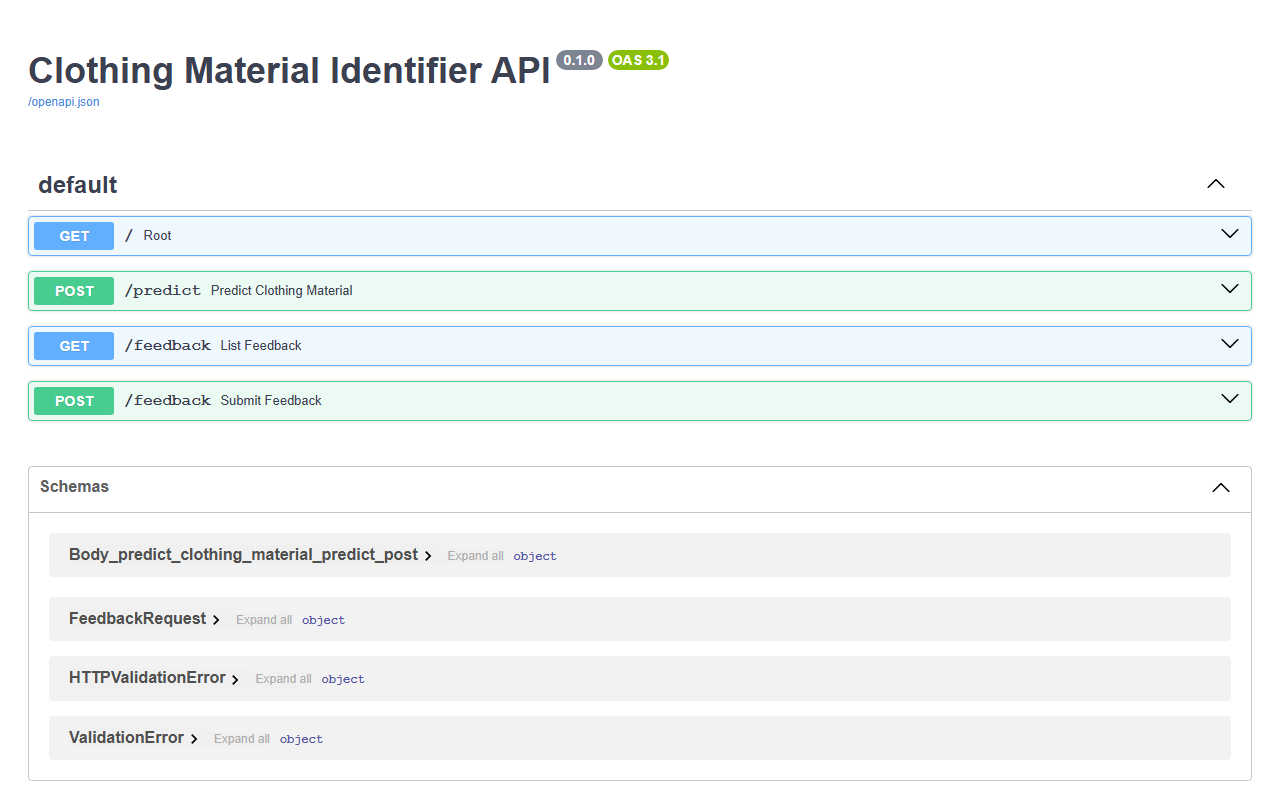
\includegraphics[width=0.9\textwidth]{img/c5diagram5}
    \caption{FastAPI 1 Documentation at \url{http://localhost:8000/docs}}
    \label{fig:api1_docs}
\end{figure}

The documentation provides:
\begin{itemize}
    \item Interactive endpoint testing
    \item Request/response schemas
    \item Example requests
    \item Try-it-yourself functionality
\end{itemize}

\begin{figure}[H]
    \centering
    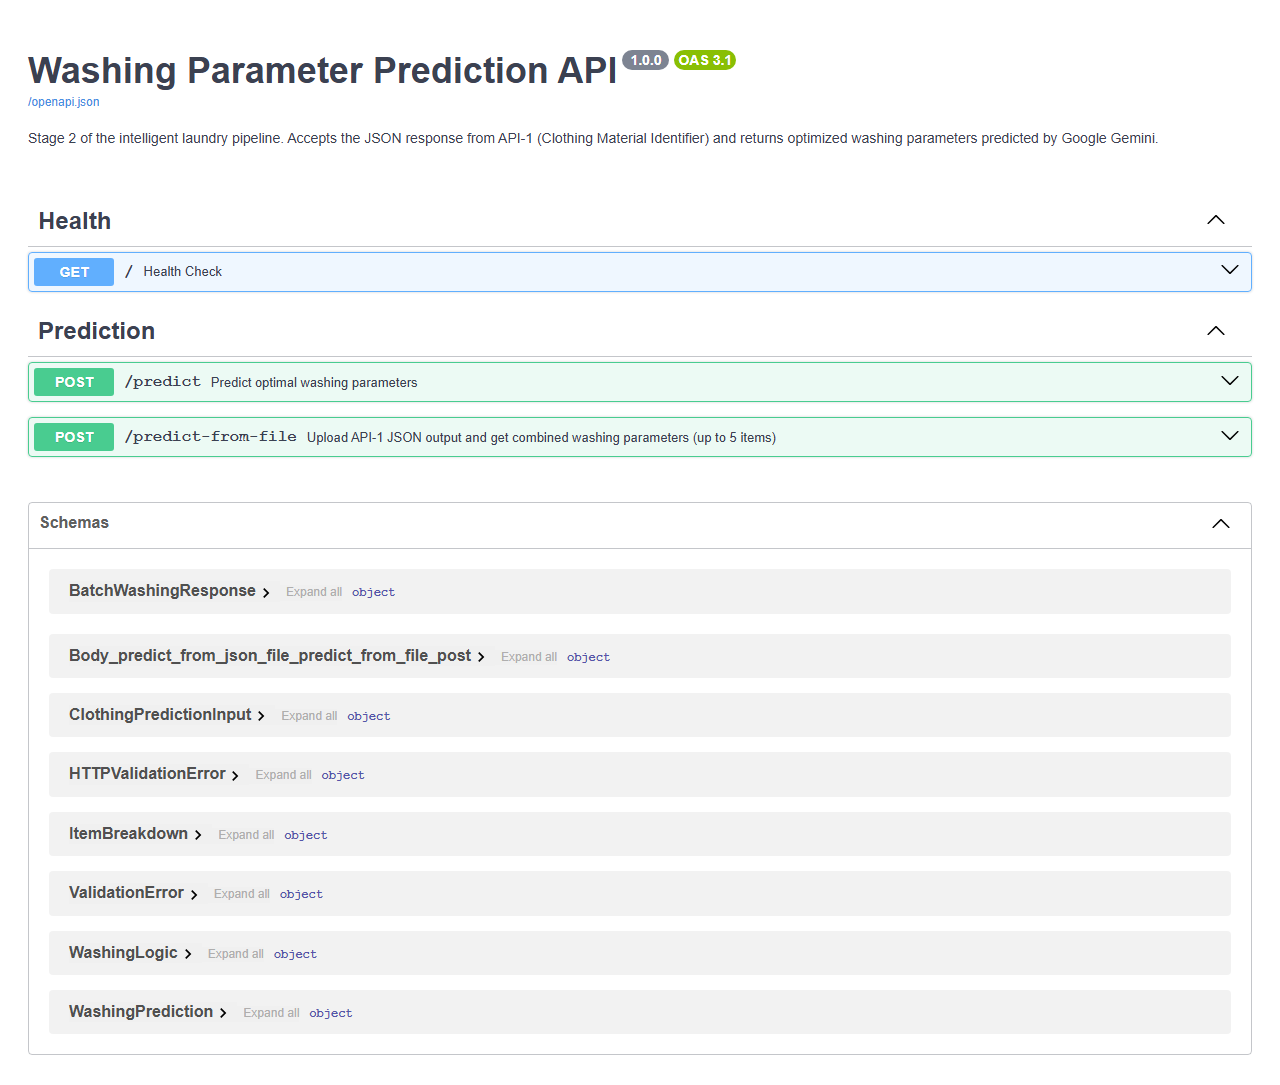
\includegraphics[width=0.9\textwidth]{img/c5diagram6}
    \caption{FastAPI 2 Documentation at \url{http://localhost:8001/docs}}
    \label{fig:api2_docs}
\end{figure}

\subsection{FastAPI 2: Washing Parameter Predictor}

\begin{lstlisting}[language=Python, caption=FastAPI 2 Code, label=lst:fastapi2]
from fastapi import FastAPI, HTTPException
from pydantic import BaseModel
from typing import List
import numpy as np

app = FastAPI(title="Washing Parameter Predictor API")

class FabricAnalysis(BaseModel):
    material_type: str
    fiber_category: str
    description: str
    dirt_level: int
    confidence_score: float

class WashParameters(BaseModel):
    temperature_setting: int
    water_level: float
    detergent_amount: float
    soak_time: int
    spin_time: int
    mechanical_action: str

class BatchWashRequest(BaseModel):
    total_images: int
    results: List[FabricAnalysis]

@app.post("/predict/", response_model=WashParameters)
async def predict_parameters(request: BatchWashRequest):
    """
    Calculate optimal washing parameters for mixed fabric loads.
    Uses safety-first algorithm prioritizing most delicate items.
    """
    analyses = request.results
    
    # Extract parameters from each analysis
    temps = []
    spins = []
    dirt_levels = []
    actions = []
    
    for item in analyses:
        # Map fabric category to base temperature
        if item.fiber_category == "Natural":
            base_temp = 40
        elif item.fiber_category == "Synthetic":
            base_temp = 30
        else:  # Semi-synthetic
            base_temp = 35
            
        # Adjust based on dirt level
        temp_adjustment = min(item.dirt_level * 2, 10)
        temps.append(base_temp + temp_adjustment)
        
        # Spin time based on fabric category
        if item.fiber_category == "Natural":
            spins.append(12 if "Denim" in item.material_type else 10)
        elif item.fiber_category == "Synthetic":
            spins.append(6)
        else:
            spins.append(8)
        
        dirt_levels.append(item.dirt_level)
        
        # Mechanical action
        if "Silk" in item.material_type or "Chiffon" in item.material_type:
            actions.append("Gentle")
        elif "Denim" in item.material_type or "Cotton" in item.material_type:
            actions.append("Heavy Duty")
        else:
            actions.append("Normal")
    
    # SAFETY FIRST: Take minimum values for delicate items
    safe_temperature = min(temps)
    safe_spin_time = min(spins)
    
    # Calculate water based on number of items (cap at 60L)
    water_per_item = 15  # Base liters per item
    calculated_water = len(analyses) * water_per_item
    water_level = min(calculated_water, 60)
    
    # Detergent based on highest dirt level
    max_dirt = max(dirt_levels)
    base_detergent = 20  # ml baseline
    detergent_amount = base_detergent + (max_dirt * 5)
    
    # Select gentlest mechanical action
    action_priority = {"Gentle": 1, "Normal": 2, "Heavy Duty": 3}
    gentlest_action = min(actions, key=lambda a: action_priority[a])
    
    return {
        "temperature_setting": safe_temperature,
        "water_level": water_level,
        "detergent_amount": detergent_amount,
        "soak_time": max_dirt * 5,  # 5 minutes per dirt level
        "spin_time": safe_spin_time,
        "mechanical_action": gentlest_action
    }
\end{lstlisting}


\newpage
\section{AI Integration}

\subsection{Prompt Engineering}
The prompts sent to Gemini were carefully engineered to ensure consistent, structured responses.

\begin{figure}[H]
    \centering
    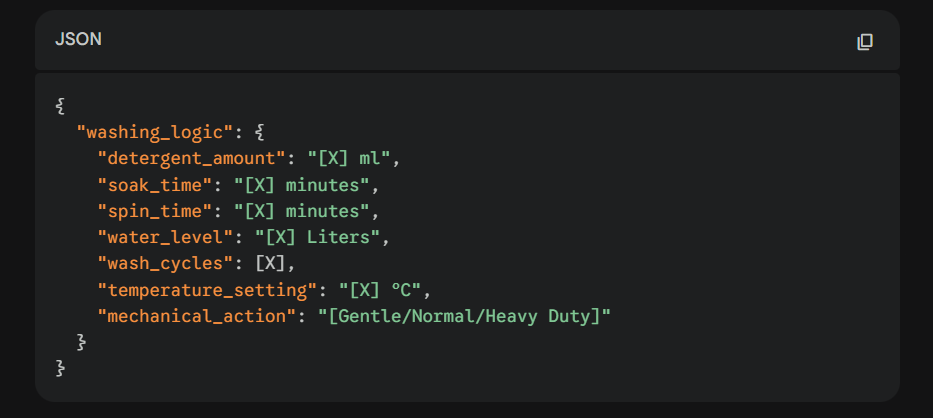
\includegraphics[width=0.9\textwidth]{img/c5diagram7}
    \caption{Example Prompt Screenshot}
    \label{fig:prompt_screenshot}
\end{figure}

\textbf{Prompt 1 (Fabric Analysis):}
\begin{verbatim}
Objective: Look at this photo of clothing.

1. Tell me the specific fabric name (like Cotton, Silk, Denim, Polyester).
2. Tell me if it's Natural, Synthetic, or Semi-synthetic.
3. Tell me how dirty it is on a scale of 1 to 5 using these criteria:
   Level 1: Clean/Light Use - No visible stains
   Level 2: Surface Soiled - Localized minor spots
   Level 3: Moderately Dirty - Visible sweat marks or multiple small stains
   Level 4: Heavily Soiled - Large deep-set stains covering >25% of surface
   Level 5: Emergency - Complete saturation with thick grime
4. Provide a 3-line description of the fabric properties including:
   - Durability and strength
   - Breathability and comfort
   - Care requirements

Return the answer in strict JSON format with keys: 
material_type, fiber_category, description, dirt_level, confidence_score
\end{verbatim}

\textbf{Prompt 2 (Washing Parameters):}
\begin{verbatim}
Based on this fabric analysis:
- Material: {material_type}
- Fiber Category: {fiber_category}
- Dirt Level: {dirt_level}

Calculate optimal washing machine parameters:
1. Temperature setting (degC) - Safe for this fabric
2. Water level (liters) - Based on single item (15L base)
3. Detergent amount (ml) - Base 20ml + 5ml per dirt level
4. Soak time (minutes) - 5 minutes per dirt level
5. Spin time (minutes) - Delicate: 6, Normal: 8-10, Heavy: 12
6. Mechanical action (Gentle/Normal/Heavy Duty)

Return in JSON format.
\end{verbatim}

\subsection{Example AI Response}

\begin{figure}[H]
    \centering
    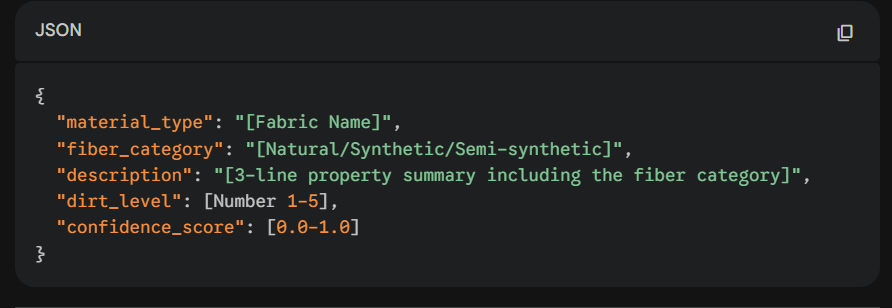
\includegraphics[width=0.9\textwidth]{img/c5diagram8}
    \caption{Example JSON Response Screenshot}
    \label{fig:ai_response}
\end{figure}

\begin{lstlisting}[language=JSON, caption=Gemini API JSON Response]
{
  "material_type": "Cotton Denim",
  "fiber_category": "Natural",
  "description": "Highly durable diagonal twill weave fabric. Excellent breathability with good moisture absorption. Moderate wrinkle resistance requiring ironing for crisp appearance.",
  "dirt_level": 4,
  "confidence_score": 0.94
}
\end{lstlisting}

\newpage
\subsection{Rate Limiting and Error Handling}

\begin{lstlisting}[language=Python, caption=Retry Logic for Gemini API, label=lst:retry]
from tenacity import retry, stop_after_attempt, wait_exponential
import google.api_core.exceptions

@retry(
    stop=stop_after_attempt(3),
    wait=wait_exponential(multiplier=1, min=2, max=10),
    retry=google.api_core.exceptions.ResourceExhausted
)
def call_gemini_with_retry(prompt, image):
    """Call Gemini API with automatic retry on rate limit"""
    try:
        response = model.generate_content([prompt, image])
        return response
    except Exception as e:
        print(f"API call failed: {e}")
        raise
\end{lstlisting}

\section{Hardware Execution}

\subsection{Complete Hardware Setup}
The Arduino is connected to the existing washing machine components through the relay modules and motor drivers.

\begin{figure}[H]
    \centering
    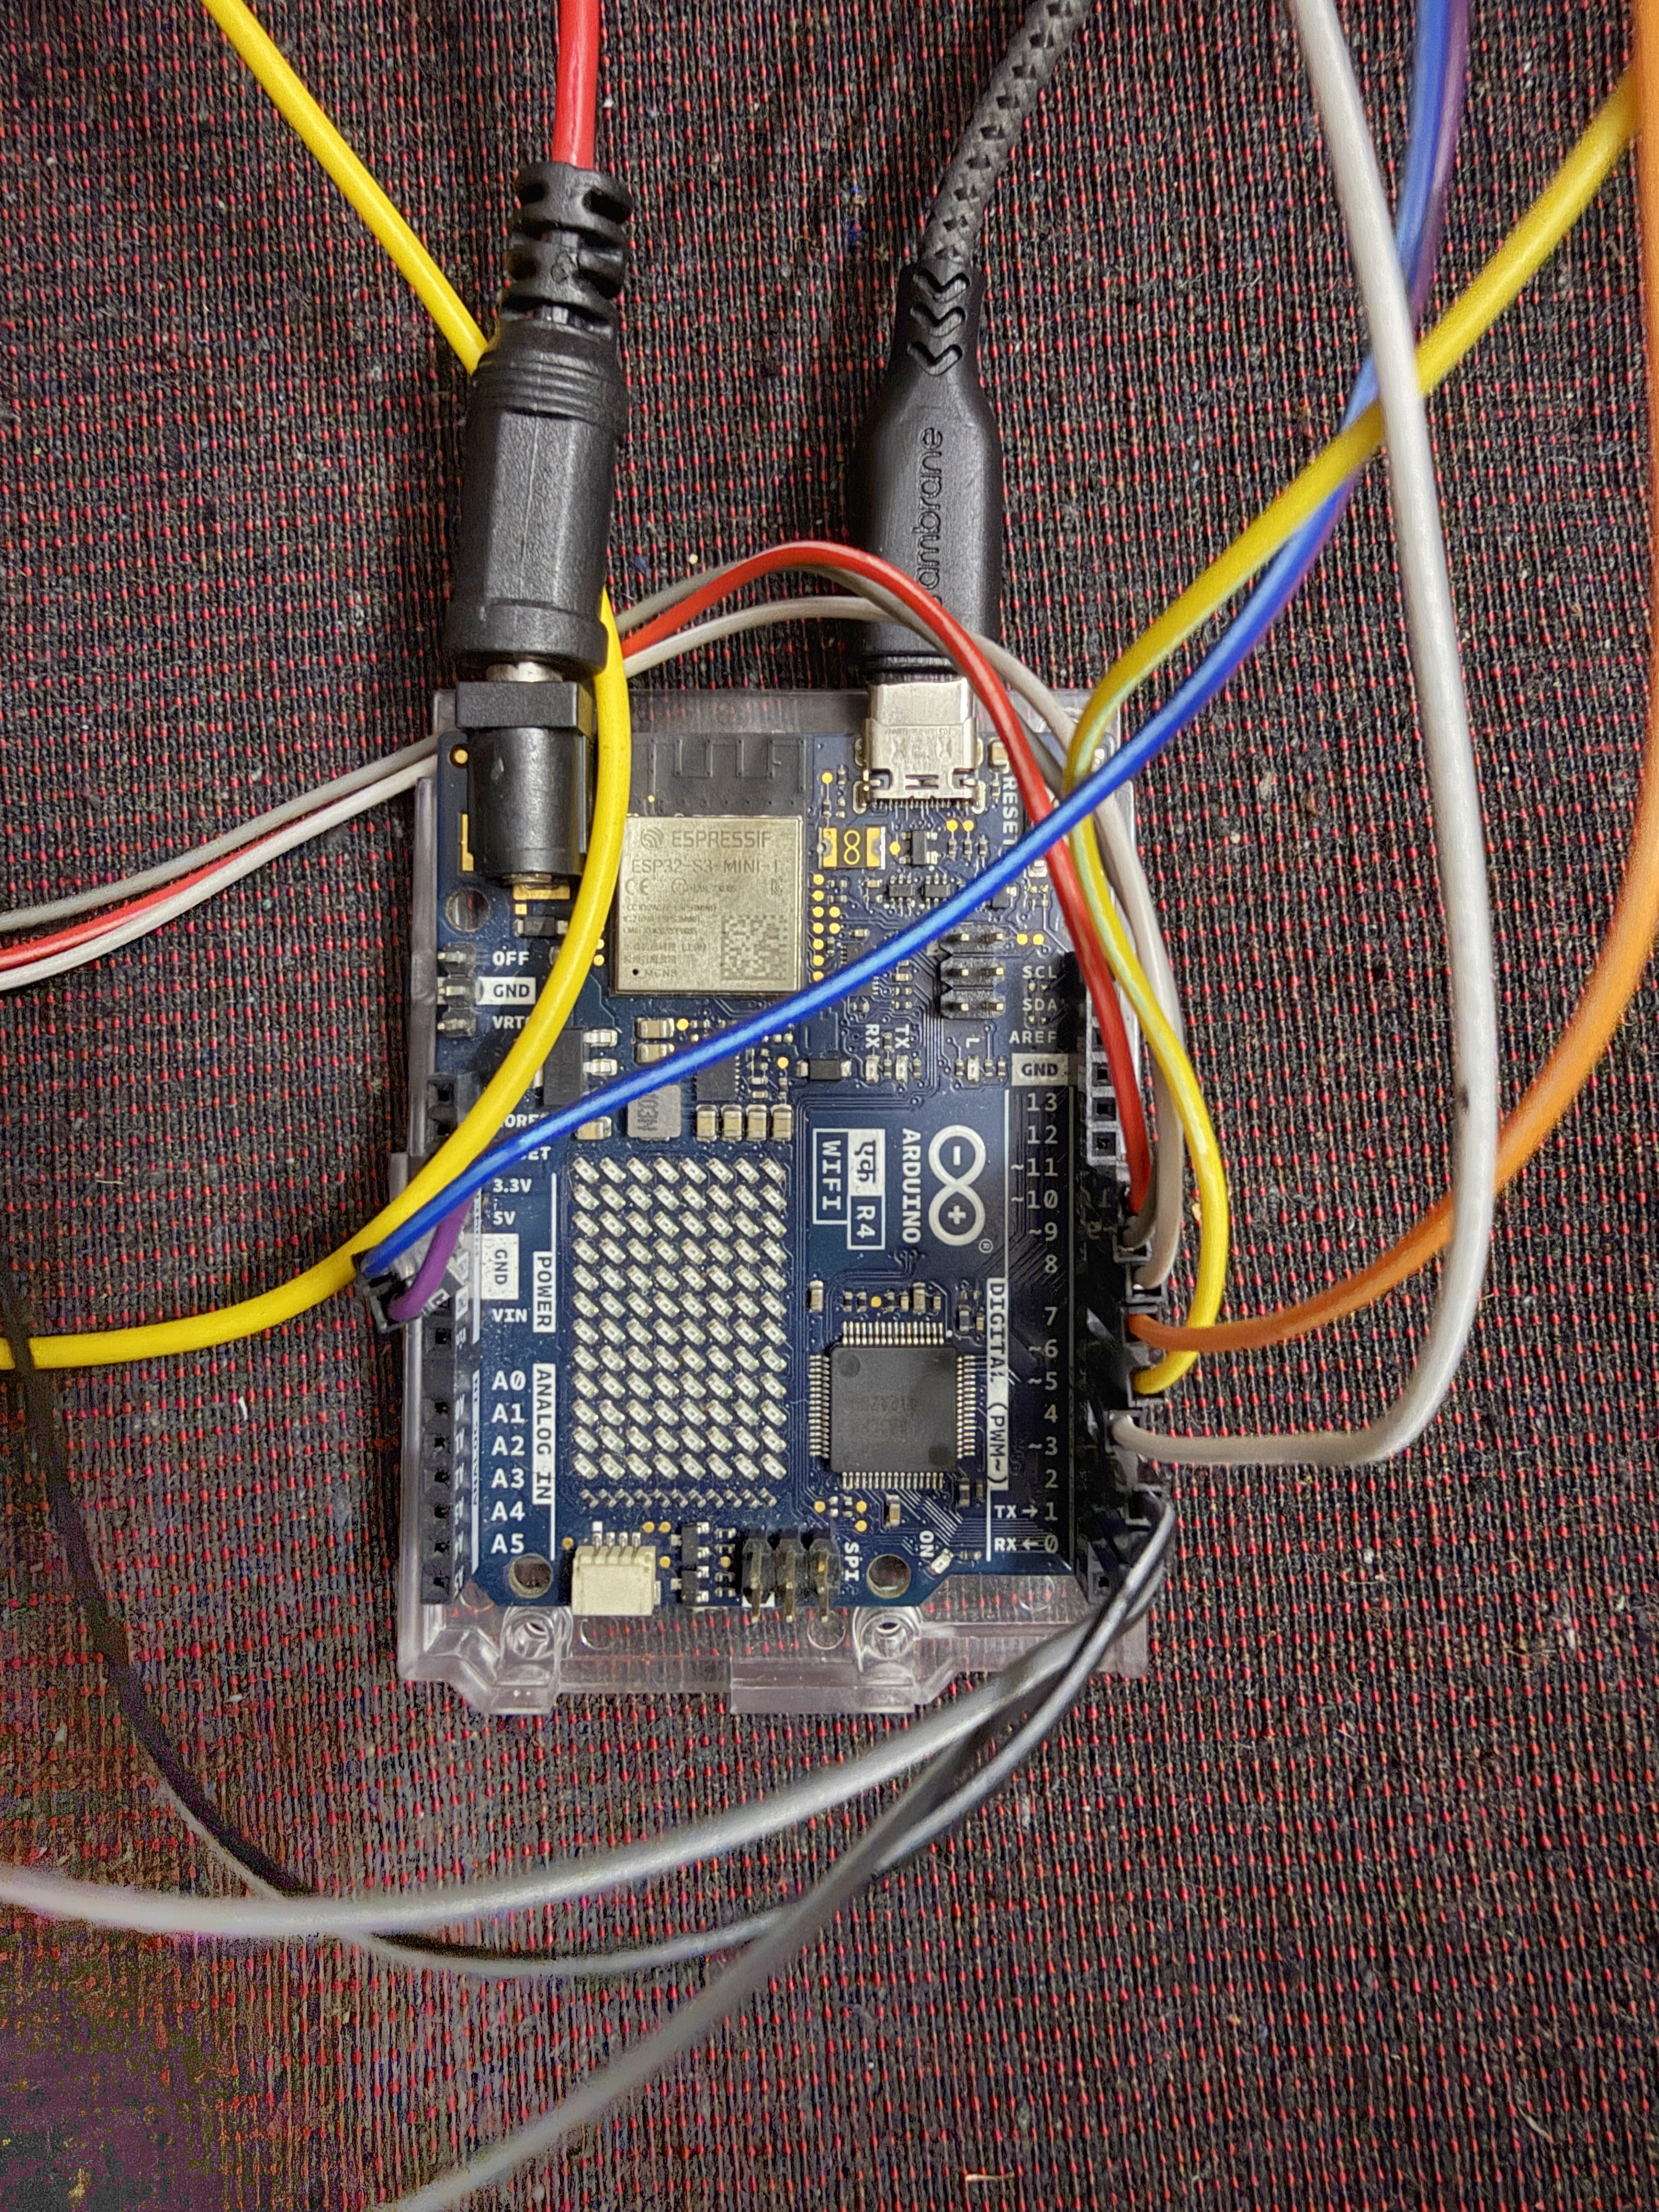
\includegraphics[width=0.45\textwidth, angle=90]{img/c5diagram9}
    \caption{Arduino WiFi R4 Connected to Washing Machine Control Panel}
    \label{fig:arduino_connected}
\end{figure}

\newpage
The image shows:
\begin{itemize}[noitemsep, topsep=0pt]
    \item Arduino WiFi R4 mounted securely
    \item Wiring harness to relays and sensors
    \item Connection to existing machine wiring
    \item Power supply for logic circuits
\end{itemize}

\subsection{Relay Control Module}
Two relays control the 240V AC motor for direction switching, while a third relay controls the water inlet solenoid.

\begin{figure}[H]
    \centering
    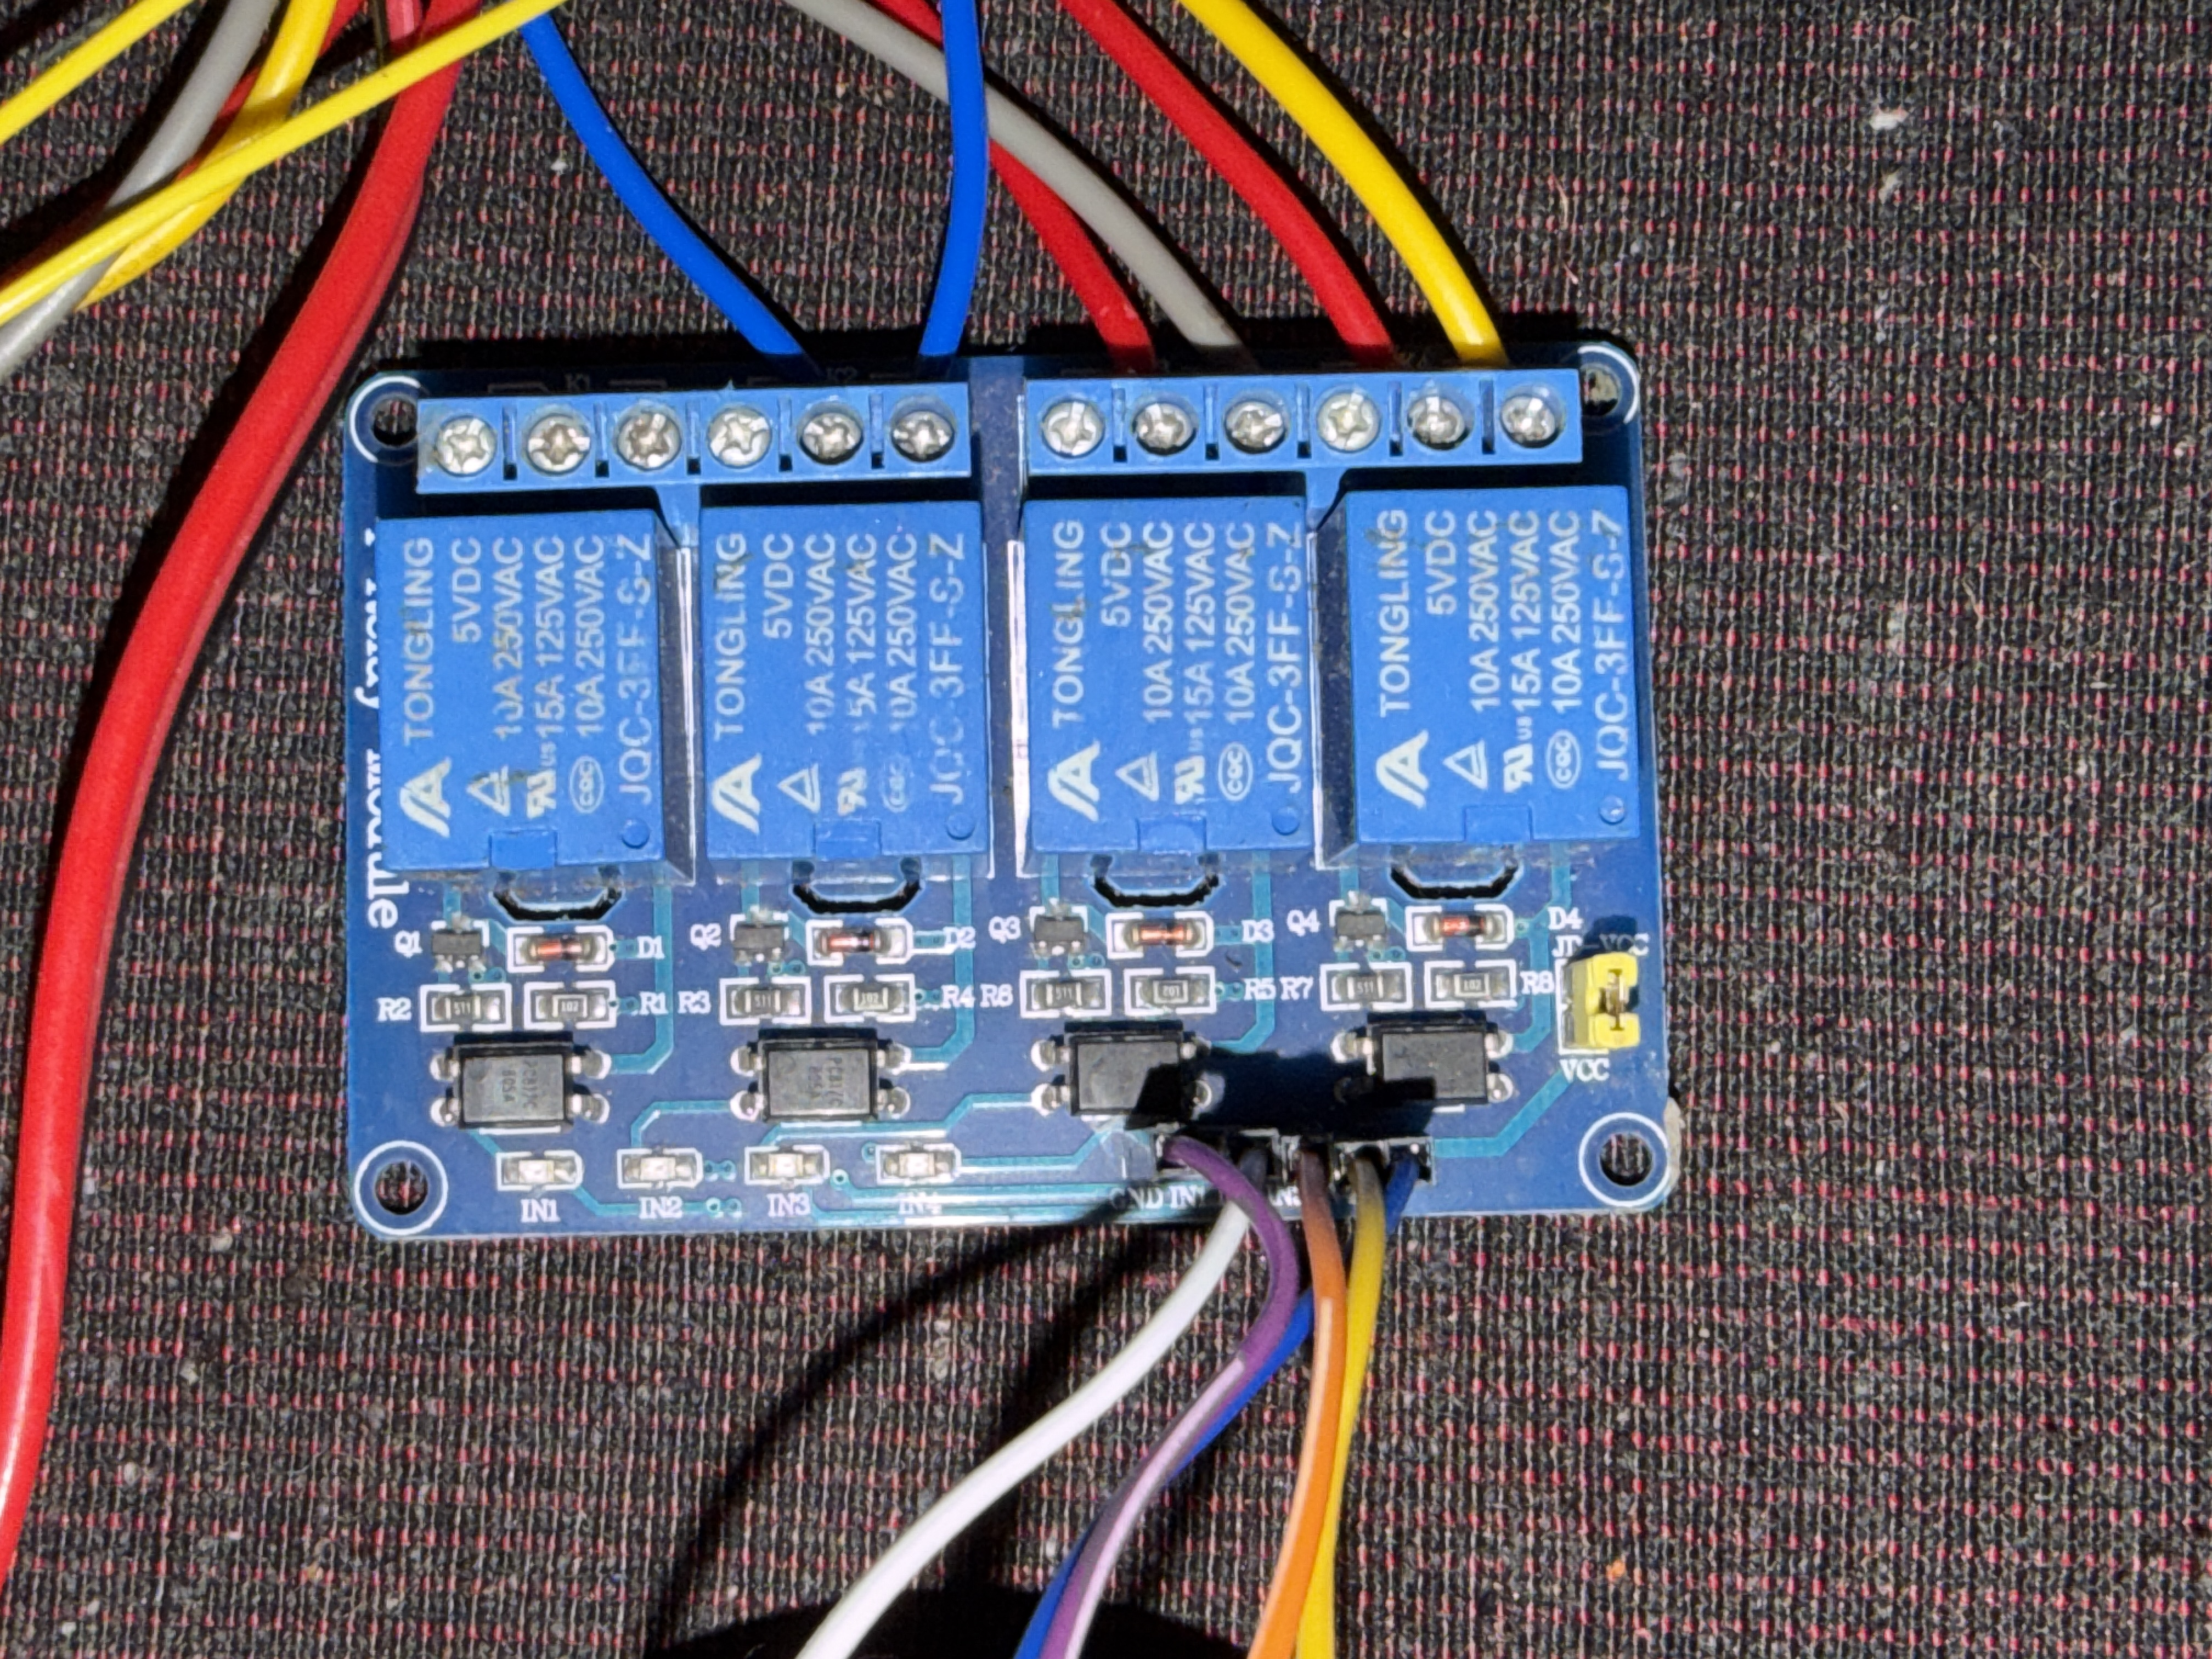
\includegraphics[width=0.9\textwidth]{img/c5diagram10}
    \caption{3-Channel Relay Module for Motor and Water Control}
    \label{fig:relay_module}
\end{figure}

\begin{table}[H]
    \centering
    \begin{tabular}{|c|c|c|}
        \hline
        \textbf{Relay} & \textbf{Function} & \textbf{Rating} \\
        \hline
        Relay 1 & Motor Clockwise & 240V AC, 10A \\
        Relay 2 & Motor Counter-Clockwise & 240V AC, 10A \\
        Relay 3 & Water Inlet Solenoid & 240V AC, 5A \\
        \hline
    \end{tabular}
    \caption{Relay Functions}
    \label{tab:relays}
\end{table}

\subsection{Detergent Dispenser Pump}
The 5V DC pump draws liquid detergent from a container and dispenses it directly into the washing drum.

\begin{figure}[H]
    \centering
    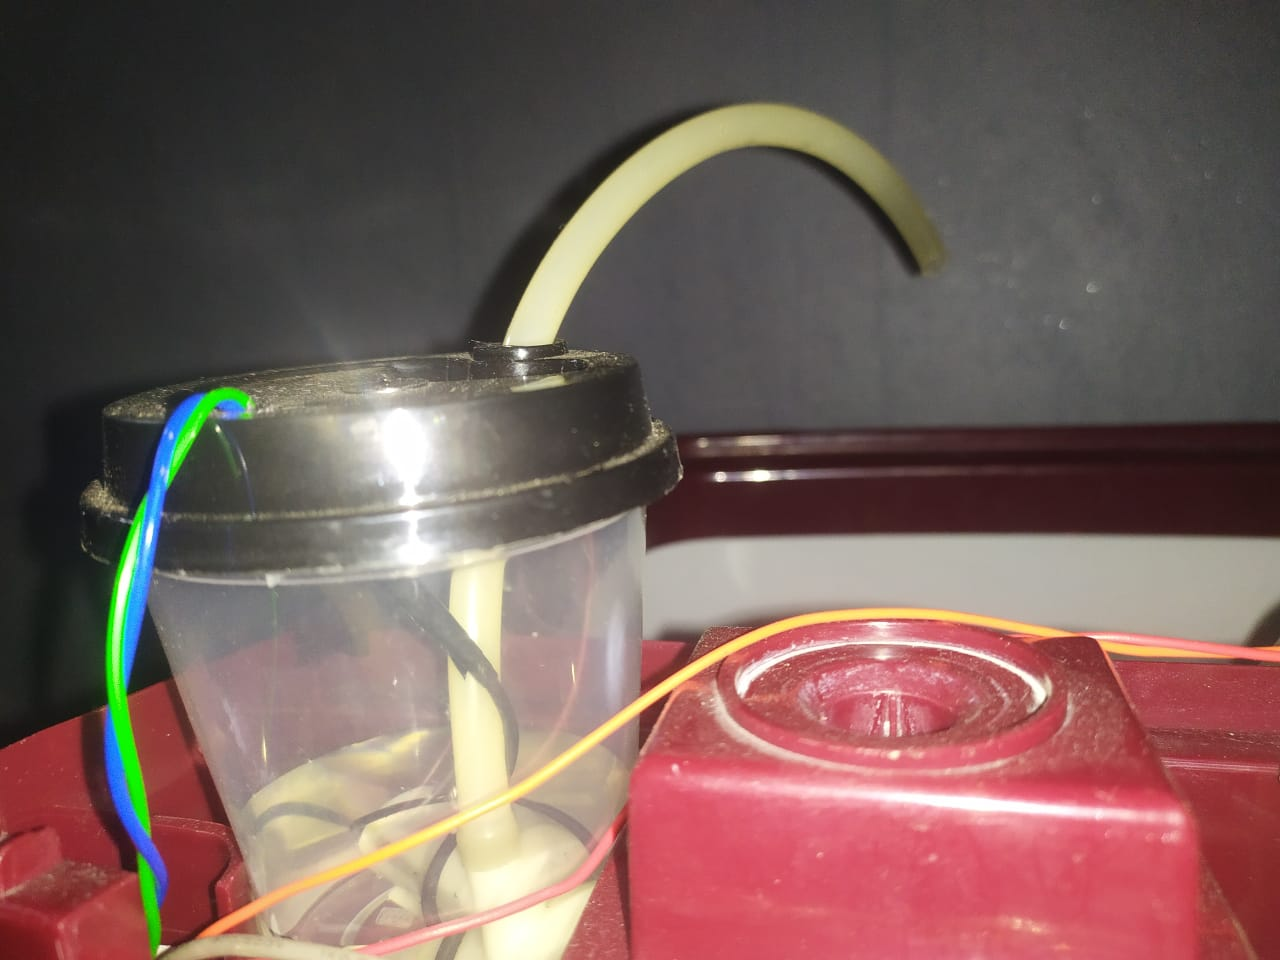
\includegraphics[width=0.9\textwidth]{img/c5diagram11}
    \caption{5V DC Pump with Motor Driver Control}
    \label{fig:pump}
\end{figure}

\textbf{Components:}
\begin{itemize}
    \item 5V DC water pump
    \item Motor driver (e.g., L298N) or H-bridge
    \item 1N4007 flyback diode
    \item Silicone tubing
    \item Detergent container
\end{itemize}

\textbf{Operation:}
The pump is activated for precise durations calculated by the linear regression formula, delivering exact detergent volumes.

\newpage
\subsection{Water Inlet Solenoid Valve}
The solenoid valve controls water flow from the household supply into the washing machine drum.

\begin{figure}[H]
    \centering
    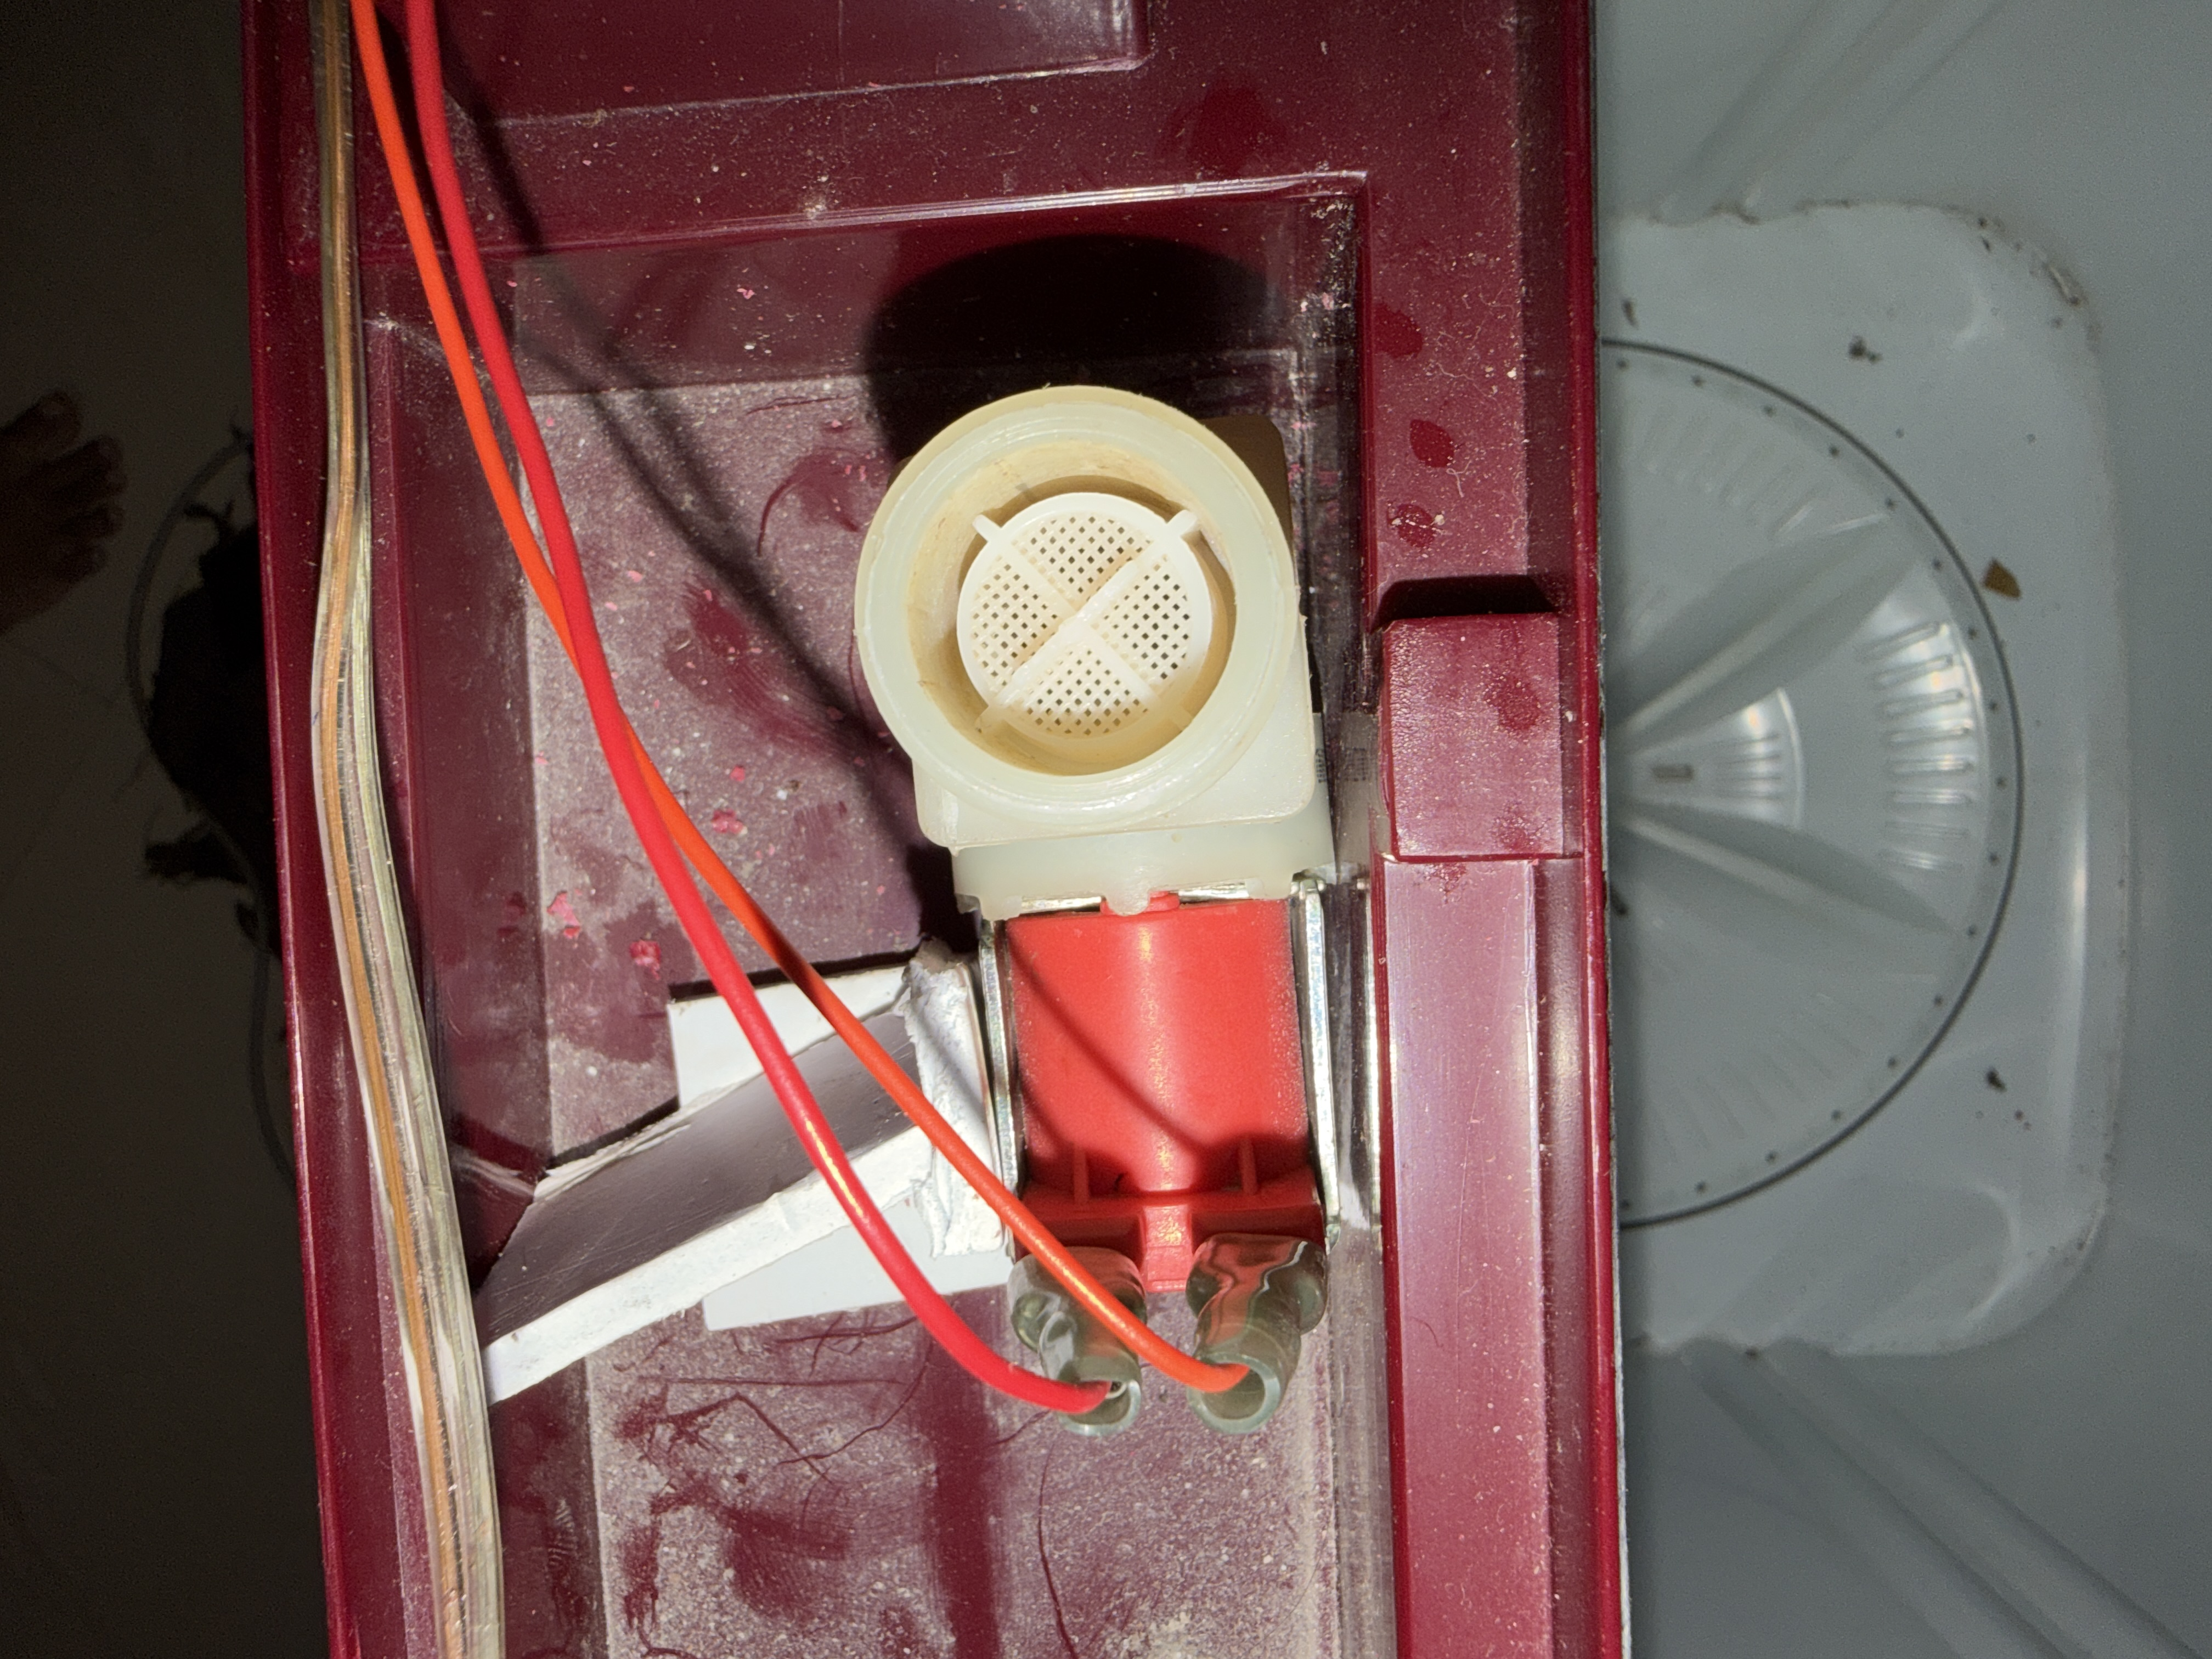
\includegraphics[width=0.9\textwidth]{img/c5diagram12}
    \caption{240V AC Solenoid Water Inlet Valve}
    \label{fig:solenoid}
\end{figure}

\textbf{Specifications:}
\begin{itemize}
    \item Voltage: 240V AC
    \item Normally closed (opens when energized)
    \item Flow rate: 8 L/min at standard pressure
    \item Connection: 3/4" threaded inlet/outlet
\end{itemize}

\subsection{Complete Wiring Diagram Implementation}
The physical implementation follows the circuit design from Chapter 4, with all components connected according to the pin mapping:

\begin{table}[H]
    \centering
    \begin{tabular}{|c|l|c|}
        \hline
        \textbf{Arduino Pin} & \textbf{Component} & \textbf{Connection} \\
        \hline
        D2 & Pump Driver & IN2 \\
        D3 & Pump Driver & IN1 \\
        D5 (PWM) & Pump Driver & EN \\
        D6 & Relay (Water Inlet) & Signal \\
        D7 & Relay (Motor CW) & Signal \\
        D8 & Relay (Motor CCW) & Signal \\
        D9 & Outlet Motor Driver & IN1 \\
        D10 & Outlet Motor Driver & IN2 \\
        D11 (PWM)& Outlet Motor Driver & ENA \\
        5V & Relay modules / Drivers & VCC \\
        GND & All components & Common ground \\
        \hline
    \end{tabular}
    \caption{Arduino Pin Mapping}
    \label{tab:pinmap}
\end{table}

\section{End-to-End Integration Testing}
A complete test was performed to validate the entire system from image capture to hardware execution.

\subsection{Test Execution Log}

\begin{small}
\begin{verbatim}
============================================================
TEST START: Intelligent Laundry System End-to-End
============================================================

STEP 1: Image Capture
- Image: denim_jeans.jpg
- Resolution: 1920x1080
- Format: JPEG
- Status: SUCCESS

STEP 2: API 1 - Fabric Analysis
- Endpoint: http://localhost:8000/predict/
- Response Time: 2.3 seconds
- Status: SUCCESS

Response:
{
  "material_type": "Cotton Denim",
  "fiber_category": "Natural",
  "dirt_level": 4,
  "confidence_score": 0.94
}

STEP 3: API 2 - Parameter Calculation
- Endpoint: http://localhost:8001/predict/
- Response Time: 0.15 seconds
- Status: SUCCESS

Response:
{
  "temperature_setting": 40,
  "water_level": 15,
  "detergent_amount": 40,
  "soak_time": 20,
  "spin_time": 12,
  "mechanical_action": "Heavy Duty"
}

STEP 4: Arduino Execution
- Parameters received via WiFi
- Detergent calculation: Time = (40 + 3.569687) / 0.022176 = 1964 ms
- Water fill: 15L @ 8 L/min = 1.875 minutes = 112.5 seconds
- Motor pattern: Heavy Duty (8s CW, 1s pause, 8s CCW)
- Status: Cycle started

============================================================
TEST RESULT: PASSED - System fully operational
============================================================
\end{verbatim}
\end{small}

\section{Implementation Summary}

\begin{table}[H]
    \centering
    \begin{tabular}{|l|c|c|p{5cm}|}
        \hline
        \textbf{Component} & \textbf{Technology} & \textbf{Status} & \textbf{Key Feature} \\
        \hline
        Microcontroller & Arduino WiFi R4 & Implemented & Real-time control with WiFi \\
        Motor Control & 2x Relays & Implemented & 5s CW / 2s pause / 5s CCW pattern \\
        Detergent Dispensing & 5V DC Pump + Transistor & Implemented & Linear regression precision \\
        Water Inlet & Solenoid Valve + Relay & Implemented & Time-based volume control \\
        Water Outlet & L298N + DC Motor & Implemented & Automated drainage \\
        API 1 & FastAPI + Gemini & Implemented & Fabric analysis with feedback \\
        API 2 & FastAPI & Implemented & Mixed-load safety algorithm \\
        Mobile App & React Native & Implemented & User interface (see Chapter 6) \\
        \hline
    \end{tabular}
    \caption{Implementation Summary}
    \label{tab:impl_summary}
\end{table}